\documentclass[DONG_CHAY_NEN_DUOC.tex]{subfiles}

\begin{document}
\chapter{SÓNG XUNG KÍCH NGHIÊNG}
\section{Giới thiệu}
Như trong chương trước, chúng ta đã xử lý sóng xung kích xiên như là những sự gián đoạn. Do đó ở đây, ta không quan tâm đến cấu trúc bên trong của song xung kích, mà đơn giản là thiết lập các mối quan hệ bước nhảy liên kết giữa trạng thái trước, sau sóng xung kích và trạng thái sóng xung kích xiên. Các kỹ thuật được sử dụng ở đây giống với các kỹ thuật đã được sử dụng ở chương trước đó. Các hệ thức đối với sóng xung kích thẳng vẫn có giá trị đối với sóng xung kích xiên nếu như chúng ta thay số Mach ở trước sóng xung kích bởi thành phần trực chuẩn của nó. Ngược lại, nghiệm hoàn chỉnh của bài toán có thể đôi khi phức tạp hơn, và cần phải có một thói quen giải bài toán này nhanh để xác định phương pháp giải được sử dụng. Các sóng xung kích xiên hiện diện nhiều trong một số rất lớn các cấu hình, và chúng ta có thể nói từ quan điểm thực nghiệm rằng, đối với dòng chảy siêu thanh, trường hợp không xuất hiện sóng xung kích xiên là rất hiếm (Hình 3.1.).
\section{Các phương trình cân bằng đối với sóng xung kích xiên}
Cấu hình mà chúng ta nghiên cứu được thể hiện trong hình 3.2. Chúng ta xết một sóng xung kích như được sinh ra từ một sự lệch dòng chảy, thí dụ như có thành uốn cong. Sóng xung kích xiên này ngăn cách miền trước sóng (kí hiệu (1)) và miền sau sóng (kí hiệu (2)). Sóng này là tĩnh, có nghĩa là nó không chuyển động trong hệ quy chiếu phòng thí nghiệm (sau này chúng ta sẽ xử lý trường hợp sóng xung kích di động). Chúng ta sẽ ký hiệu $\bfit v_1$ và $\bfit v_2$ lần lượt là vần tốc phía trước và phía sau sóng xung kích, $\epsilon$ là góc giữa $\bfit v_1$ và hướng dọc theo sóng xung kích, $\beta$ là góc giữa $\bfit v_2$ và hướng dọc theo sóng xung kích. Giá trị $\delta=\epsilon-\beta$ biểu diển sự biến đổi trong góc của dòng chảy, có nghĩa là sự lệch.\\
\begin{figure}[h!]
	\centering
	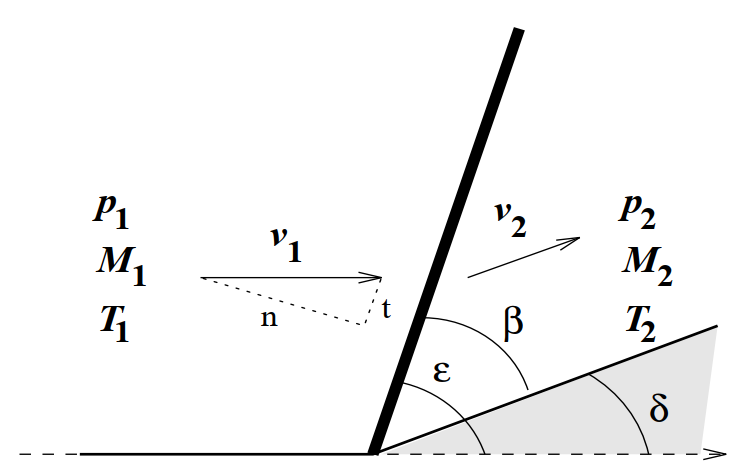
\includegraphics[scale = 0.8]{CHOC_OBLIQUE_CONFIG.png}
	\caption{Cấu hình của lưu chất khi có sự hình thành sóng xung kích xiên.}
\end{figure}


Ta kí hiệu $n$ và $t$ là thành phần trực giao và tiếp tuyến đối với một vecteur được xét. Chúng ta đặt mình trong các giả thiết sau :
\begin{itemize}
	\item không có lực nhớt cũng như lực thể tích.
	\item tất cả các đường dòng là song song với nhau.
	\item không có phản ứng hóa học cũng như sự trao đổi năng lượng với môi trường bên ngoài, và lưu chất ở trong cân bằng nhiệt động.
\end{itemize}

Như vậy, các phương trình tồn tại trong lưu chất bao gồm :
\begin{itemize}
	\item Phương trình bảo toàn khối lượng :
	\begin{equation}
		\begin{aligned}
			\rho_1 v_{n_1} = \rho_2 v_{n_2}
		\end{aligned}
	\end{equation}
	\item Phương trình bảo toàn động lượng :
	\begin{equation}
		\begin{aligned}
			p_1 + \rho_1 v_{n_1}^ 2= p_2 + \rho_2 v_{n_2}^2
		\end{aligned}
	\end{equation}
	\item Phương trình cân bằng năng lượng :
	\begin{equation}
		\begin{aligned}
			h_1 + \frac{v_{n_1}^2}{2}= 	h_2 + \frac{v_{n_2}^2}{2}
		\end{aligned}
	\end{equation}
	\item Sự liên tục của vận tốc tiếp tuyến :
	\begin{equation}
		\begin{aligned}
			v_{t_1} = v_{t_1}
		\end{aligned}
	\end{equation}
\end{itemize}

Từ các phương trình này, chúng ta thấy ở phía sau sóng xung kích, dòng bị lệch về phía sóng xung kích. Hơn nữa, phía trước sóng xung kích luôn là dòng chảy siêu thanh.
\section{Sóng xung kích xiên đối với khí lý tưởng}
Đối với khí lý tưởng, chúng ta có phương trình trạng thái $p =\rho hT$ và $h = c_pT$. Thay thế các phương trình trạng thái này vào trong các phương trình (3.1) - (3.4), chúng ta có thể định nghĩa số Mach của thành phần vận tốc trực giao (gọi tắt là số Mach trực giao) :
\begin{equation}
	\begin{aligned}
		\boxed{
			M_{n1} = M_1 \sin\epsilon
		}
	\end{aligned}
\end{equation}

Từ đây, chúng ta có thể \bfit{áp dụng các phương trình đã biết đối với sóng xung kích thẳng} với điều kiện là phải \bfit{thay thế số Mach thông thường bởi số Mach trực giao}. Tuy nhiên, chúng ta cần một phương trình để xác định quan hệ hình học giữa sóng xung kích và các dòng chảy. Đầu tiên, các quan hệ vận tốc tiếp tuyến cho ta (xem Hình 3.1):
$$
\frac{{{\rho _2}}}{{{\rho _1}}} = \frac{{{v_{1n}}}}{{{v_{2n}}}} = \frac{{{v_{1t}}\tan \epsilon }}{{{v_{2t}}\tan \left( {\epsilon  - \delta } \right)}} = \frac{{\tan \epsilon }}{{\tan \left( {\epsilon  - \delta } \right)}}.
$$
Kết hợp với phương trình xác định khối lượng riêng (...) đã biết ở chương 2, chúng ta có :
$$
\frac{{\tan \epsilon }}{{\tan \left( {\epsilon  - \delta } \right)}} = \frac{{\left( {\gamma  + 1} \right)M_1^2{{\sin }^2}\epsilon }}{{2 + \left( {\gamma  - 1} \right)M_1^2{{\sin }^2}\epsilon }}
$$

Do đó khi khai triển hàm tan và sắp xếp lại các số hạng, chúng ta có một hệ thức quan trong sau để xác định quan hệ hình học :
\begin{equation}
	\begin{aligned}
		\boxed{
			\frac{1}{{\tan \delta }} = \left( {\frac{{\gamma  + 1}}{2}\frac{{M_1^2}}{{M_1^2{{\sin }^2}\epsilon  - 1}} - 1} \right)\tan \epsilon 
		}
	\end{aligned}
\end{equation}
\section{Sự bất định giữa sóng xung kích yếu và mạnh}
Với cùng một số Mach trước xung kích $M_1$ và với cùng một góc lệch $\delta$, chúng ta có thể xác định được hai góc $\epsilon$ từ phương trình (3.6) (và do đó là hai giá trị số Mach ở sau sóng xung kích $M_2$). Giá trị $\epsilon$ lớn hơn úng với trường hợp sóng xung kích mạnh và phía sau sóng xung kích là dòng chảy hạ âm, trường hợp ngược lại ứng với sóng xung kích yếu. Đối với sóng xung kích yếu, nếu không rơi vào một số trường hợp đặc biệt của $M_1$ và $\delta$, dòng chảy phía sau sóng xung kích là dòng chảy siêu âm.

Không có phương pháp tuyệt đối nào để xác định đối với một cấu hình dòng chảy cho trước, sóng xung kích xiên sinh ra là mạnh hoặc yếu. Tuy nhiên, bằng thực nghiệm, người ta thấy rằng trong phần lớn các trường hợp, dòng chảy phía sau sóng xung kích ứng với sóng xung kích yếu, đặc biệt là khi sóng xung kích "dính" vào thành vật cản. Sóng xung kích mạnh là cực kỳ hiếm xảy ra, và nó xuất hiện điển hình trong trường hợp sóng xung kích tách hoàn toàn khỏi bề mặt.
\section{Sóng xung kích cực yếu}
Khi mà góc lệch $\delta$ là nhỏ, chúng ta thu được một sóng xung kích gần như là thẳng (sóng xung kích rất mạnh). Chúng ta nghiên cứu trường hợp này bằng cách xấp xỉ : $\tan \delta \simeq \delta$. Các hệ thức khác nhau sẽ được biểu diển trong khuôn khổ của xấp xỉ này, chúng ta chú ý hệ thức quan trọng sau :
\begin{equation}
	\begin{aligned}
		\boxed{
			\frac{{\Delta v}}{{{v_1}}} =  - \frac{1}{{{{\left( {M_1^2 - 1} \right)}^{1/2}}}}\delta
		}
	\end{aligned}
\end{equation}
\section{Sóng Mach}
Giống như đối với sóng xung kích thẳng, sóng xung kích nghiêng tồn tại nếu như số Mach trực chuẩn là siêu thanh, tức là $M_1\sin\epsilon \ge 1$. Điều này ngụ ý rằng lưu chất đang trong chế độ siêu thanh. Nhưng trong trường hợp giới hạn $M_1\sin\epsilon = 1$, dựa vào hệ thức (4.20), chúng ta suy ra $\delta = 0$. Tức là ta nói chất khí không chịu bất kỳ một sự đổi hướng nào. Sóng xung kích nghiêng do đó được gọi là sóng Mach. Hướng của sóng được xác định theo quan hệ : $\sin \epsilon = 1/M_1$, nhiệt độ, áp suất, khối lượng riêng và vận tốc chịu một sự biến đổi vô cùng nhỏ dọc theo đường này :
\begin{equation}
	\begin{aligned}
		\frac{p_1}{p_2}=\frac{v_1}{v_2}=\frac{T_2}{T_1} = 1.
	\end{aligned}
\end{equation}

Do đó, chúng ta tìm được một góc tương đương với cấu hình này được gọi là góc Mach, kí hiệu là $\mu$. Không tồn tại sóng xung kích nghiêng trong chế độ ổn định nếu như dòng chảy trước sóng xung kích có một góc nhỏ hơn $\mu$
\begin{equation}
	\begin{aligned}
		\boxed{
			\mu = \arcsin\Bigg(\frac{1}{M_1}\Bigg)
		}
	\end{aligned}
\end{equation}

Các đường Mach do đó là những đường thẳng có góc tới là $\pm \mu$ theo hướng cục bộ của dòng. Trong các chương tiếp theo, chúng ta sẽ tìm hiểu làm thế nào để sử dụng đường Mach để tìm đặc trưng của các cấu hình phức tạp hơn.
\section{Cực xung kích}
Cực xung kích là một phương pháp nhanh và hữu ích để hình tượng hóa một vài hiện tượng tương tác. Để bắt đầu, chúng ta hãy xét một dòng chảy mà vận tốc $\bfit v_2$ thay đổi sau khi có một sóng xung kích nghiêng đối với vận tốc $\bfit v_1$ cho trước, mà ta thay đổi góc của sóng xung kích $\epsilon$. Chúng ta áp dụng công thức bên trên. Chúng ta biết $v_1$ và $T_1$, do đó $M_1$, và góc của sóng xung kích $\epsilon$, chúng ta tính toán số Mach trực giao $M_{n1}$. Chúng ta có thể tính toán tỉ lệ $T_2/T_1$ thông qua công thức (...) và chúng ta có thể suy ra $T_2$. Mặc khác, chúng ta biết $M_1$ và góc $\epsilon$ có thể xác định ngay lập tức $\delta$ thông qua (...). Chúng ta có thể tính toán số Mach trực giao ở phía sau sóng xung kích $M_{n2}$ qua (...), chúng ta có thể xác định số Mach phía sau thông qua $M_2 = M_{n2}/\sin(\epsilon-\delta)$. Chúng ta tính toán trực tiếp vận tốc phía sau sóng xung kích xiên thông qua $v_2=M_2\sqrt{\gamma rT_2}$. Chúng ta có thể thu được Hình 4 . Đường cong $(\mathcal{C})$ mô tả thông qua một đầu của vecteur vận tốc $\bfit v_2$ khi chúng ta thay đổi góc $\epsilon$ được gọi là cực xung kích. Đường cong này cần một vài bình luận.






	
\end{document}